\documentclass[11pt,a4paper]{article}
\usepackage{acl2015}
\usepackage{times}
\usepackage{latexsym}
% \setlength\titlebox{5cm}    % Expanding the titlebox

%%% Custom additions %%%
% \usepackage{hyperref}
\usepackage{url}
\usepackage[leqno, fleqn]{amsmath}
\usepackage{amssymb}
\usepackage{qtree}
\usepackage{graphicx}
\usepackage{booktabs}
\usepackage{multirow}
\usepackage{colortbl}
\usepackage{caption}
\usepackage{subcaption}
\usepackage{color}
\usepackage{xcolor}
\usepackage{tikz}
\usepackage{ifthen}
\usepackage{framed}

\hyphenation{Verb-Ocean}

% abbreviations
\def\eg{\emph{e.g.}}
\def\Eg{\emph{E.g.}}
\def\etal{\emph{et al.}}

% names - lowercase
\newcommand{\fracnet}{FractalNet}
\newcommand{\fracnets}{FractalNets}
\newcommand{\resnet}{ResNet}
\newcommand{\resnets}{ResNets}
\newcommand{\dropout}{dropout}
\newcommand{\dropconn}{drop-connect}
\newcommand{\droppath}{drop-path}

% names - uppercase
\newcommand{\Fracnet}{FractalNet}
\newcommand{\Fracnets}{FractalNets}
\newcommand{\Resnet}{ResNet}
\newcommand{\Resnets}{ResNets}
\newcommand{\Dropout}{Dropout}
\newcommand{\Dropconn}{Drop-connect}
\newcommand{\Droppath}{Drop-path}


\newcount\colveccount
\newcommand*\colvec[1]{
        \global\colveccount#1
        \begin{bmatrix}
        \colvecnext
}
\def\colvecnext#1{
        #1
        \global\advance\colveccount-1
        \ifnum\colveccount>0
                \\
                \expandafter\colvecnext
        \else
                \end{bmatrix}
        \fi
}


\newcommand{\nateq}{\equiv}
\newcommand{\natind}{\mathbin{\#}}
%\newcommand{\natneg}{\raisebox{2px}{\tiny\thinspace$\wedge$\thinspace}}
\newcommand{\natneg}{\mathbin{^{\wedge}}}
\newcommand{\natfor}{\sqsubset}
\newcommand{\natrev}{\sqsupset}
\newcommand{\natalt}{\mathbin{|}}
\newcommand{\natcov}{\mathbin{\smallsmile}}

\newcommand{\plneg}{\mathop{\textit{not}}}
\newcommand{\pland}{\mathbin{\textit{and}}}
\newcommand{\plor}{\mathbin{\textit{or}}}

% Strikeout
\newlength{\howlong}\newcommand{\strikeout}[1]{\settowidth{\howlong}{#1}#1\unitlength0.5ex%
\begin{picture}(0,0)\put(0,1){\line(-1,0){\howlong\divide\unitlength}}\end{picture}}

\newcommand{\True}{\texttt{T}}
\newcommand{\False}{\texttt{F}}
\usepackage{stmaryrd}
\newcommand{\sem}[1]{\ensuremath{\llbracket#1\rrbracket}}

\newcommand{\mynote}[1]{{\color{blue}#1}}

\newcommand{\tbchecked}[1]{{\color{red}#1}}

\usepackage{gb4e}
\noautomath
 
 
\def\ii#1{\textit{#1}}
\newcommand{\word}[1]{\emph{#1}}
\newcommand{\fulllabel}[2]{\b{#1}\newline\textsc{#2}}

%%%%%%%%%%%%%%%%%%%%%%%%%%%%%%%%%%%%%%%%%%%%%%%%%%%%%%%%%%%%%%%%%%%%%%
%%%%% Code to simulate natbib's citealt, which prints citations with
%%%%% no parentheses:

\makeatletter
\def\citealt{\def\citename##1{{\frenchspacing##1} }\@internalcitec}
\def\@citexc[#1]#2{\if@filesw\immediate\write\@auxout{\string\citation{#2}}\fi
  \def\@citea{}\@citealt{\@for\@citeb:=#2\do
    {\@citea\def\@citea{;\penalty\@m\ }\@ifundefined
       {b@\@citeb}{{\bf ?}\@warning
       {Citation `\@citeb' on page \thepage \space undefined}}%
{\csname b@\@citeb\endcsname}}}{#1}}
\def\@internalcitec{\@ifnextchar [{\@tempswatrue\@citexc}{\@tempswafalse\@citexc[]}}
\def\@citealt#1#2{{#1\if@tempswa, #2\fi}}
\makeatother

%%%%%%%%%%%%%%%%%%%%%%%%%%%%%%%%%%%%%%%%%%%%%%%%%%%%%%%%%%%%%%%%%%%%%%


%%% %%%

\title{A large annotated corpus for learning natural language inference}

\author{
Samuel R.\ Bowman$^{\ast\dag}$ \\
\texttt{sbowman@stanford.edu} \\
\And
Gabor Angeli$^{\dag\ddag}$ \\
\texttt{angeli@stanford.edu} \\
\AND
Christopher Potts$^{\ast}$\\
\texttt{cgpotts@stanford.edu}
\And
Christopher D.\ Manning$^{\ast\dag\ddag}$\\
\texttt{manning@stanford.edu}\\
\AND\\[-3ex]
{$^{\ast}$Stanford Linguistics\quad
$^{\dag}$Stanford NLP Group\quad
$^{\ddag}$Stanford Computer Science}
}

\date{}

\makeatletter
\newcommand{\@BIBLABEL}{\@emptybiblabel}
\newcommand{\@emptybiblabel}[1]{}
\definecolor{black}{rgb}{0,0,0}
\makeatother
\usepackage[breaklinks, colorlinks, linkcolor=black, urlcolor=black, citecolor=black]{hyperref}

\def\t#1{#1}
\def\b#1{\t{\textbf{#1}}}
\def\colspaceS{2.25mm}
\def\colspaceM{4.0mm}
\def\colspaceL{4.25mm}

\begin{document}
\maketitle

\begin{abstract}

We propose a convolutional neural network (CNN) architecture for facial expression recognition. The proposed architecture is independent of any hand-crafted feature extraction and performs better than the earlier proposed convolutional neural network based approaches. We visualize the automatically extracted features which have been learned by the network in order to provide a better understanding. The standard datasets, i.e. Extended Cohn-Kanade (CKP) and MMI Facial Expression Databse are used for the quantitative evaluation. On the CKP set the current state of the art approach, using CNNs, achieves an accuracy of 99.2\%. For the MMI dataset, currently the best accuracy for emotion recognition is 93.33\%. The proposed architecture achieves $99.6$\% for CKP and $98.63$\% for MMI, therefore performing better than the state of the art using CNNs. Automatic facial expression recognition has a broad spectrum of applications such as human-computer interaction and safety systems. This is due to the fact that non-verbal cues are important forms of communication and play a pivotal role in interpersonal communication. The performance of the proposed architecture endorses the efficacy and reliable usage of the proposed work for real world applications.

\end{abstract}

%\cite{burger2001issues}
%\cite{fader2014open}
%\cite{voorhees1999trec}


%A huge leap forward in artificial intelligence will be achieved when
%machines will be able to answer any question expressed in natural
%language. As such, q

Question answering (QA) has been a long standing research problem in
natural language processing, with the first systems attempting to
answer questions by directly reading
documents \citep{voorhees2000building}. The development of large-scale Knowledge Bases (KBs) such as Freebase  \citep{bollacker2008freebase}
helped organize information into structured forms, prompting recent progress to focus on answering questions by converting them into logical forms that can be used to query such databases \citep{berant2013semantic,kwiatkowski-EtAl:2013:EMNLP,fader2014open}.

Unfortunately, KBs have intrinsic limitations such as their inevitable incompleteness and fixed schemas that cannot support all varieties of answers.
%
Since information extraction (IE) \citep{craven2000learning}, intended to
fill in missing information in KBs, is neither accurate nor
reliable enough, collections of raw textual resources and
documents such as Wikipedia will always contain more information.
%than KBs.
%
As a result, even if KBs can be satisfactory for closed-domain problems, they are unlikely
to scale up to answer general questions on any
topic.
%
Starting from this observation,
%here we propose  to study the problem
in this work we study the problem
of answering by directly reading documents.


Retrieving answers directly from text is harder than
from KBs because information is far less structured, is
indirectly and ambiguously expressed, and is usually scattered across multiple documents.
%
%This explains why, when a satisfactory KB is
%available -- which is typically only the case in closed domains --
%using it instead of raw text is preferred. %, because performance is better.
%
This explains why using a satisfactory KB---typically only available in closed domains---is preferred over raw text.
%
We postulate that before trying to provide answers that are not in
KBs, document-based QA systems should first reach KB-based systems'
performance in such closed domains, where clear comparison and
evaluation is possible.
%
To this end, this paper introduces {\sc WikiMovies}, a new
analysis tool that allows for measuring the performance of %loss induced on
QA systems when the knowledge source is switched from a KB to unstructured documents.
%
{\sc WikiMovies} contains $\sim$100k questions in the movie domain, and was designed
to be answerable by using either a perfect KB
(based on OMDb\footnote{\url{http://www.omdbapi.com}}), Wikipedia pages or an imperfect KB obtained through
running %a standard IE pipeline on those pages.
an engineered IE pipeline on those pages.

To bridge the gap between using a KB and reading documents directly,
we still lack appropriate machine learning algorithms. In this
work we propose the Key-Value Memory Network (KV-MemNN), a new neural network
architecture that generalizes the original Memory Network
\citep{sukhbaatar2015end} and can work with either knowledge source.
%
The KV-MemNN performs QA by first storing facts in a key-value
structured memory before reasoning on them in order to predict an
answer. The memory is designed so that the model learns to use keys to
address relevant memories with respect to the question, whose corresponding values are subsequently returned.
%
This structure allows the model to encode prior knowledge for the considered task
and to leverage possibly complex transforms between keys and values,
while still being trained using standard backpropagation via
stochastic gradient descent.

Our experiments on {\sc WikiMovies} indicate that, thanks to its key-value memory,
the KV-MemNN consistently outperforms the
original Memory Network, and reduces the gap between answering from a human-annotated KB,
from an automatically extracted KB or from directly reading Wikipedia.
%
We confirm our findings on  {\sc WikiQA} \citep{yang2015wikiqa},
another Wikipedia-based QA benchmark where no KB is available,
where we demonstrate that KV-MemNN can reach state-of-the-art results---surpassing
the most recent attention-based neural network models.

% Note: The examples have been moved to the previous section in order to appear on p. 2.

\section{A new corpus for NLI}\label{sec:discussion}

To date, the primary sources of annotated NLI corpora have been the
Recognizing Textual Entailment (RTE)
challenge tasks.\footnote{\url{http://aclweb.org/aclwiki/index.php?title=Textual_Entailment_Resource_Pool}}
These are generally high-quality, hand-labeled data sets, and they
have stimulated innovative logical and statistical models of natural
language reasoning, but their small size (fewer than a thousand examples each)
limits their utility as a testbed for learned distributed representations. 
The data for the SemEval 2014 task called Sentences Involving Compositional Knowledge (SICK) is a step up in terms of size, but only to 4,500 training examples, and its
partly automatic construction introduced some spurious patterns into
the data (\citealt{marelli2014semeval}, $\S$6). The
Denotation Graph entailment set \cite{hodoshimage} contains millions of
examples of entailments between sentences and artificially constructed
short phrases, but it was labeled using fully automatic methods, and is
noisy enough that it is probably suitable only as a source of
supplementary training data.
Outside the domain of sentence-level entailment, \newcite{levy2014focused} introduce
a large corpus of semi-automatically annotated entailment examples 
between subject--verb--object relation triples, and the second release of the 
Paraphrase Database \cite{ganitkevitch2ppdb} includes automatically generated entailment annotations
over a large corpus of pairs of words and short phrases.

Existing resources suffer from a subtler issue that impacts even
projects using only human-provided annotations: indeterminacies of
event and entity coreference lead to insurmountable indeterminacy
concerning the correct semantic label (\citealt{de2008finding} $\S4.3$; \citealt{marelli2014sick}). 
For an example of the pitfalls surrounding entity coreference, consider the sentence pair \word{A boat sank in the Pacific Ocean} and \word{A boat sank in the Atlantic Ocean}. The pair could be labeled as a contradiction if one assumes that the two sentences refer to the same single event, but could also be reasonably labeled as neutral if that assumption is not made. In order to ensure that our labeling scheme assigns a single correct label to every pair, we must select one of these approaches across the board, but both choices present problems. If we opt not to assume that events are coreferent, then we will only ever find contradictions between sentences that make broad universal assertions, but if we opt to assume coreference, new counterintuitive predictions emerge. For example, \ii{Ruth Bader Ginsburg was appointed to the US Supreme Court} and \ii{I had a sandwich for lunch today} would unintuitively be labeled as a contradiction, rather than neutral, under this assumption.

Entity coreference presents a similar kind of indeterminacy, as in the pair \word{A tourist visited New York} and \word{A tourist visited the city}. Assuming coreference between \ii{New York} and \ii{the city} justifies labeling the pair as an entailment, but without that assumption \ii{the city} could be taken to refer to a specific unknown city, leaving the pair neutral. This kind of indeterminacy of label can be resolved only once the questions of coreference are resolved.

With SNLI, we sought to address the issues of size, quality, and
indeterminacy. To do this, we employed a crowdsourcing framework with
the following crucial innovations. First, the examples were grounded
in specific scenarios, and the premise and hypothesis sentences in each example 
were constrained to describe that scenario from the same perspective, 
which helps greatly in controlling event and entity coreference.\footnote{
Issues of coreference are not completely solved, but greatly mitigated. For example, with the premise sentence \word{A dog is lying in the grass}, a worker could safely assume that the dog is the most prominent thing in the photo, and very likely the only dog, and  build contradicting sentences assuming reference to the same dog.
} 
Second, the prompt
gave participants the freedom to produce entirely novel sentences
within the task setting, which led to richer examples than we see with
the more proscribed string-editing techniques of earlier approaches,
without sacrificing consistency. Third, a subset of the resulting
sentences were sent to a validation task aimed at providing a highly 
reliable set of annotations over the same data, and at identifying areas of inferential uncertainty.

% Our ultimate aim in this work is to develop supervised models for sentence representation that can accurately capture natural language meaning. While sentiment tasks like SST have provided a useful testbed for sentence representation models, sentiment labeling only requires that models be able to encode a small piece of the full expressive capacity of language. We claim that the task of natural language inference (also called recognizing textual entailment, or RTE) is significantly more demanding, and that strong performance on this task is good evidence of a model's overall strength in sentence representation.

% \subsection{Grounding with imagined images}

% Quote from SICK paper \cite{marelli2014sick}:

% \begin{quote}
% Not unreasonably, subjects found that, say, \ii{A woman is wearing an Egyptian headdress} does not contradict \ii{A woman is wearing an Indian headdress}, since one could easily imagine both sentences truthfully uttered to refer to a single scene where two different women are wearing different headdresses. In the future, a higher proportion of CONTRADICTION labels could be elicited by using grammatical and possibly visual cues (pictures) encouraging co-indexing of the entities in the two sentences.
% \end{quote}

\subsection{Data collection}

\begin{figure}
\begin{framed}
\small
We will show you the caption for a photo. We will not show you the photo. Using only the caption and what you know about the world:
\begin{itemize}
\item Write one alternate caption that is \textbf{definitely} a \textbf{true} description of the photo. \ii{Example: For the caption ``\ii{Two dogs are running through a field.}'' you could write ``\ii{There are animals outdoors.}"}
\item Write one alternate caption that \textbf{might be} a \textbf{true} description of the photo. \ii{Example: For the caption ``\ii{Two dogs are running through a field.}" you could write ``\ii{Some puppies are running to catch a stick.}"}
\item Write one alternate caption that is \textbf{definitely} a \textbf{false} description of the photo. \ii{Example: For the caption ``\ii{Two dogs are running through a field.}" you could write ``\ii{The pets are sitting on a couch.}" This is different from the} maybe correct \ii{category because it's impossible for the dogs to be both running and sitting.}
\end{itemize}
\end{framed}

\caption{\label{instructions-1}The instructions used on Mechanical Turk for data collection.}
\end{figure}

We used Amazon Mechanical Turk for data collection. In each individual task (each HIT), a worker was presented with premise scene descriptions from a pre-existing corpus, and asked to supply hypotheses for each of our three labels---\ii{entailment}, \ii{neutral}, and \ii{contradiction}---forcing the data to be balanced among these classes.

The instructions that we provided to the workers are shown in \reffig{instructions-1}. Below the instructions were three fields for each of three requested sentences, corresponding to our \ii{entailment}, \ii{neutral}, and \ii{contradiction} labels, a fourth field (marked optional) for reporting problems, and a link to an FAQ page. That FAQ grew over the course of data collection. It warned about disallowed techniques (e.g., reusing the same sentence for many different prompts, which we saw in a few cases), provided guidance concerning sentence length and complexity (we did not enforce a minimum length, and we allowed bare NPs as well as full sentences), and reviewed logistical issues around payment timing. About 2,500 workers contributed.

For the premises, we used captions from the Flickr30k corpus \cite{hodoshimage}, a collection of approximately 160k captions (corresponding to about 30k images) collected in an earlier crowdsourced effort.\footnote{
We additionally include about 4k sentence pairs from a pilot study in which the premise sentences were instead drawn from the VisualGenome corpus (under construction; \texttt{\href{https://visualgenome.org/}{visualgenome.org}}). These examples appear only in the training set, and have pair identifiers prefixed with \texttt{vg} in our corpus.
 } % TODO: Insert citation.
The captions were not authored by the photographers who took the source images, and they tend to contain relatively literal scene descriptions that are suited to our approach, rather than those typically associated with personal photographs (as in their example: \word{Our trip to the Olympic Peninsula}). In order to ensure that the label for each sentence pair can be recovered solely based on the available text, we did not use the images at all during corpus collection.

\Reftab{collection-stats} reports some key statistics about the collected corpus, and \reffig{length-dist} shows the distributions of sentence lengths for both our source hypotheses and our newly collected premises. We observed that while premise sentences varied considerably in length, hypothesis sentences tended to be as short as possible while still providing enough information to yield a clear judgment, clustering at around seven words. We also observed that the bulk of the sentences from both sources were syntactically complete rather than fragments, and the frequency with which the parser produces a parse rooted with an `S' (sentence) node attests to this.

\begin{table}
\center
  %\setlength{\tabcolsep}{15pt}
  %\renewcommand{\arraystretch}{1.2}
  \begin{tabular}{l r} 
    \toprule
\multicolumn{2}{l}{\textbf{Data set sizes:}}\\
Training pairs &  550,152\\
Development pairs &  10,000\\
Test pairs & 10,000\\
\midrule
\multicolumn{2}{l}{\textbf{Sentence length:}}\\
Premise mean token count & 14.1\\
Hypothesis mean token count & 8.3 \\
\midrule
\multicolumn{2}{l}{\textbf{Parser output:}}\\
Premise `S'-rooted parses & 74.0\%\\
Hypothesis `S'-rooted parses & 88.9\%\\
Distinct words (ignoring case) & 37,026\\
    \bottomrule
  \end{tabular}
% From 1.0rc3
\caption{\label{collection-stats}Key statistics for the raw sentence pairs in SNLI\@. Since the two halves of each pair were collected separately, we report some statistics for both.} 
\end{table}


\subsection{Data validation}

In order to measure the quality of our corpus, and in order to construct maximally useful testing and development sets, we performed an additional round of validation for about 10\% of our data.
This validation phase followed the same basic form as the Mechanical Turk labeling task used to label the SICK entailment data: we presented workers with pairs of sentences in batches of five, and asked them to choose a single label for each pair. We supplied each pair to four annotators, yielding five labels per pair including the label used by the original author. The instructions were similar to the instructions for initial data collection shown in \reffig{instructions-1}, and linked to a similar FAQ\@. Though we initially used a very restrictive qualification (based on past approval rate) to select workers for the validation task, we nonetheless discovered (and deleted) some instances of random guessing in an early batch of work, and subsequently instituted a fully closed qualification restricted to about 30 trusted workers.

For each pair that we validated, we assigned a gold label. If any one of
the three labels was chosen by at least three of the five annotators, it was 
chosen as the gold label. If there was no such consensus, which
occurred in about 2\% of cases, we assigned the placeholder label `-'. 
While these unlabeled examples are included in the corpus distribution, they are
unlikely to be helpful for the standard NLI classification task, and
we do not include them in either training or evaluation in the experiments that we 
discuss in this paper.

 
\begin{figure}
\center
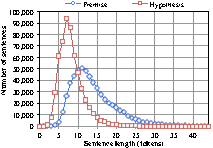
\includegraphics[width=3.05in]{length_dist}
    % From 1.0rc2, though still accurate as of rc3
\caption{\label{length-dist}The distribution of sentence length.} 
\end{figure}
 

The results of this validation process
are summarized in \reftab{validation-stats}. 
Nearly all of the examples received a majority
label, indicating broad consensus about the nature of the data and
categories. The gold-labeled examples are very nearly evenly
distributed across the three labels. The Fleiss $\kappa$ scores 
(computed over every example with a full five annotations)
are likely to be conservative given our large and
unevenly distributed pool of annotators, but they still provide insights
about the levels of disagreement across the three semantic
classes. This disagreement likely reflects not just the limitations of
large crowdsourcing efforts but also the uncertainty inherent in naturalistic NLI\@.
Regardless, the overall rate of agreement is extremely high,
suggesting that the corpus is sufficiently high quality to pose a
challenging but realistic machine learning task.

\begin{table}
\center
  %\setlength{\tabcolsep}{15pt}
  %\renewcommand{\arraystretch}{1.2}
  \begin{tabular}{l r} 
    \toprule
\multicolumn{2}{l}{\textbf{General:}}\\
Validated pairs & 56,951\\
Pairs w/ unanimous gold label & 58.3\%\\
\midrule
\multicolumn{2}{l}{\textbf{Individual annotator label agreement:}}\\
Individual label $=$ gold label & 89.0\%\\
Individual label $=$ author's label & 85.8\%\\
\midrule
\multicolumn{2}{l}{\textbf{Gold label/author's label agreement:}}\\
Gold label $=$ author's label & 91.2\%\\
Gold label $\ne$ author's label & 6.8\% \\
No gold label (no 3 labels match) & 2.0\%\\
\midrule
\multicolumn{2}{l}{\textbf{Fleiss $\kappa$:}}\\
    \ii{contradiction} & 0.77 \\
    \ii{entailment} & 0.72 \\
    \ii{neutral} & 0.60 \\
    Overall & 0.70 \\
    \bottomrule
  \end{tabular}
    % From 1.0rc3
\caption{\label{validation-stats}Statistics for the validated pairs. The \ii{author's label} is the label used by the worker who wrote the premise to create the sentence pair. A \ii{gold label} reflects a consensus of three votes from among the author and the four annotators.} 
\end{table}

\subsection{The distributed corpus}

\Reftab{snli-examples} shows a set of randomly chosen validated examples from the development set with their labels. Qualitatively, we find the data that we collected draws fairly extensively on commonsense knowledge, and that hypothesis and premise sentences often differ structurally in significant ways, suggesting that there is room for improvement beyond superficial word alignment models. We also find the sentences that we collected to be largely fluent, correctly spelled English, with a mix of full sentences and caption-style noun phrase fragments, though punctuation and capitalization are often omitted.

The corpus is available under a CreativeCommons
Attribution-ShareAlike license, the same license used for the Flickr30k source captions. It can be downloaded at:\\\href{http://nlp.stanford.edu/projects/snli/}{\texttt{nlp.stanford.edu/projects/snli/}}

\paragraph{Partition} 

We distribute the corpus with a pre-specified train/test/development split. The test and development sets contain 10k examples each. Each original ImageFlickr caption occurs in only one of the three sets, and all of the examples in the test and development sets have been validated.

\paragraph{Parses}

The distributed corpus includes parses produced by the Stanford PCFG Parser 3.5.2 \cite{klein2003accurate}, trained on the standard training set as well as on the Brown Corpus (\citealt{francis1979brown}), which we found to improve the parse quality of the descriptive sentences and noun phrases found in the descriptions. 

% Parses are available in both the standard PTB format and in the binarized unlabeled format used by tree-structured neural network models.

%\paragraph{General evaluation standards}
%While we hope that the corpus will be valuable in a variety of ways, we encourage researchers working on tools for semantic representation and inference to evaluate on our data in a uniform way: training on only the (parsed and/or unparsed) sentences included in the training set, and doing final evaluations on only the subset of the test set for which there are single gold labels.

\section{Our data as a platform for evaluation}

The most immediate application for our corpus is in developing models for the task of NLI\@. In particular, since it is dramatically larger than any existing corpus of comparable quality, we expect it to be suitable for training parameter-rich models like neural networks, which have not previously been competitive at this task. Our ability to evaluate standard classifier-base NLI models, however, was limited to those which were designed to scale to SNLI's size without modification, so a more complete comparison of approaches will have to wait for future work. In this section, we explore the performance of three classes of models which could scale readily: (i)~models from a well-known NLI system, the Excitement Open Platform; (ii)~variants of a strong but simple feature-based classifier model, which makes use of both unlexicalized and lexicalized features, and (iii)~distributed representation models, including a baseline model and neural network sequence models.

%
% EOP
%

\subsection{Excitement Open Platform models}

The first class of models is from the Excitement Open
  Platform (EOP,
  \citealt{pado2014design,magnini2014excitement})---an open source platform for RTE research.
%  which
%  is distributed alongside a number of RTE pipelines.
%
% what is EOP
EOP is a tool for quickly developing NLI systems
  while sharing components such as common lexical resources and 
  evaluation sets.
We evaluate on two algorithms included in the distribution:
  a simple edit-distance based algorithm and
  a classifier-based algorithm, the latter both in a bare form and augmented 
  with EOP's full suite of lexical resources.
%  (3) an algorithm based around tree transformations.

%% 9 systems compared against
%A number of systems have been built using the platform, 9 of them
%  applicable to English are publicly distributed with version 1.2.1
%  of the software.
%% these fall into 2 classes
%These fall into two classes of algorithms: 2 are edit distance based,
%  whereas the remaining 7 make use of different features in a
%  maximum entropy classifier.
%
%%% methodology
%%We convert the 3-way classification task in SNLI into the RTE setting
%%  by labeling both the \unknown\ and \contradiction\
%%  labels as negative entailment, and treating the \entailment\ label as
%%  the positive entailment.
%%This creates a biased dataset of 66\% negative examples.
%% we report the best results from each class
%We run the top performing edit-distance based algorithm and the top
%  performing classifier-based algorithm on our test set, as
%  determined by performance on the development set.
%Note that these models were run using the default configuration
%  with minimal tuning.
%The results should therefore be taken as a strong baseline for
%  NLI-style approaches to the problem, rather than necessarily
%  representing the state-of-the-art system's performance on the
%  task.
%%We run each of the 9 algorithms distributed with EOP on the 2-class
%%  SNLI dataset, and report results for the best edit distance 
%%  configuration and the best classifier based configuration, as
%%  determined by performance on the development set.

%
% EOP RESULTS TABLE
%

% The table
\begin{table}
\begin{center}
\def\t#1{\small{#1}}
\begin{tabular}{l@{\hskip \colspaceL}c@{\hskip \colspaceL}c@{\hskip \colspaceL}c}
\toprule
\b{System} & \b{SNLI} & \b{SICK} & \b{RTE-3} \\
\midrule
\t{Edit Distance Based}            & \t{71.9} & \t{65.4} & \t{61.9} \\
\t{Classifier Based}               & \t{72.2} & \t{71.4} & \t{61.5} \\
\t{$~~~$ + Lexical Resources} & \b{75.0} & \b{78.8} & \b{63.6} \\
%\midrule
%\t{Classifier Based (3-class)} & \t{??.?} & \t{65.6} & \t{} \\
%\t{Transformation Based} & \t{36.0} & \t{76.7} & \t{56.4} \\  % broken! At least, on SNLI...
\bottomrule
\end{tabular}
\end{center}
% The caption
\caption{
\label{tab:eopresults}
2-class test accuracy for two simple baseline systems included in the
  Excitement Open Platform, as well as SICK and RTE results for
  a model making use of more sophisticated lexical resources.
%All RTE results are 2-class accuracy.
%The transformation-based model allows for 3-class predictions on our
%  corpus and SICK; these are reported in the last row.
}
\end{table}
%
% END EOP RESULTS TABLE
%

% the best systems
Our initial goal was to better understand the difficulty of the task of classifying SNLI corpus inferences, rather than necessarily the performance of a state-of-the-art RTE system.
We approached this by running the same system on several data sets:
our own test set,
the SICK test data, and the standard RTE-3 test set \cite{giampiccolo2007third}.
We report results in \reftab{tab:eopresults}.
Each of the models was separately trained on the training set of each corpus.
%The results for RTE-3 are taken from \newcite{magnini2014excitement}.
All models are evaluated only on 2-class entailment.
To convert 3-class problems like SICK and SNLI to this setting, all instances
  of \contradiction\ and \unknown\ are converted to nonentailment.
This yields a most-frequent-class baseline accuracy of 66\% on SNLI, and 71\% on SICK\@.
This is intended primarily to demonstrate the difficulty of the task, rather than necessarily
  the performance of a state-of-the-art RTE system.
The edit distance algorithm tunes the weight of the three 
  case-insensitive edit distance operations on the training set, 
  after removing stop words.
In addition to the base classifier-based system distributed with the platform, we
  train a variant which includes information from
  WordNet \cite{miller1995wordnet} and VerbOcean
  \cite{chklovski2004verbocean}, and makes use of features
  based on tree patterns and dependency tree skeletons
  \cite{wang2007recognizing}.

%In particular, we could not evaluate models which rely on richer lexical resources or more
%  sophisticated algorithms. 
%None of the strongest Excitement Open Platform models
%  are designed to scale to large training corpora without modification, 
%  and none of them succeeded at training on the full SNLI training set, with no 
%  model showing any measurable progress after several days.
%We include the performance of one such model on the SICK and RTE-3 datasets to
%  gauge its relative performance.
  
%We train these models without using any of the included lexical
%  resources, so these results do not represent state-of-the-art
%  RTE systems, but rather give an indication of the relative
%  difficulties of the datasets.

%The best edit distance algorithm tunes the weight of the three 
%  case-insensitive edit distance operations on the training set, 
%  after removing stop words.
%The best classifier-based system makes use of information from
%  WordNet \cite{miller1995wordnet} and VerbOcean
%  \cite{chklovski2004verbocean}, and makes use of features
%  based on tree patterns and dependency tree skeletons
%  \cite{wang2007recognizing}.
%Unsurprisingly, the classification-based approach outperforms simple
%  edit distance metrics, and performs quite well despite relatively
%  little lexicalization.

%
% Lexicalized Classifier
%
\subsection{Lexicalized Classifier}
Unlike the RTE datasets, SNLI's size supports approaches which make use of rich lexicalized features.
We evaluate a simple lexicalized classifier to explore the ability of non-specialized models to exploit these features in lieu of more involved language understanding.
Our classifier implements 6 feature types; 3 unlexicalized and 3 lexicalized:
\begin{enumerate}
\setlength\itemsep{-0.25em}
  \item The BLEU score of the \hypothesis\ with respect
  to the \premise, using an n-gram length between 1 and 4.

  \item The length difference between the \hypothesis\ and the \premise, as a real-valued
  feature.

  \item The overlap between words in the \premise\ and \hypothesis,
  both as an absolute count and a percentage of possible overlap, and both over 
  all words and over just nouns, verbs, adjectives, 
  and adverbs.
  
  \item\label{lst:ngram} An indicator for every unigram and bigram in the \hypothesis.

  \item\label{lst:unigram} Cross-unigrams: for every pair of words across the \premise\ and \hypothesis\ which share a 
  POS tag, an indicator feature over the two words.
  
  \item\label{lst:bigram} Cross-bigrams: for every pair of bigrams across the \premise\ and \hypothesis\ which share a 
  POS tag on the second word, an indicator feature over the two bigrams.
\end{enumerate}

%
% BOW RESULTS TABLE
%

% The table
\begin{table}
\begin{center}
\begin{tabular}{l@{\hskip \colspaceL}c@{\hskip \colspaceS}c@{\hskip \colspaceL}c@{\hskip \colspaceS}c}
\toprule
\b{System}	 & \multicolumn{2}{c}{\hspace{-1.2em}\b{SNLI}} & \multicolumn{2}{c}{\b{SICK}}\\
 & \t{Train} & \t{Test} & \t{Train} & \t{Test}\\
\midrule
\t{Lexicalized}            & \t{99.7}  & \b{78.2} & \t{90.4} & \b{77.8} \\ % & \t{78.7}
\t{Unigrams Only}          & \t{93.1} & \t{71.6}  & \t{88.1} & \t{77.0} \\ % & \t{72.2}
\t{Unlexicalized}          & \t{49.4} & \t{50.4}  & \t{69.9} & \t{69.6} \\ % & \t{50.1} % Last value was 50.39; rounded for consistency.
\bottomrule
\end{tabular}
\end{center}
% The caption
\caption{
\label{tab:bowresults}
3-class accuracy, training on either our data or SICK, including models lacking cross-bigram features 
  (Feature \ref{lst:bigram}), and lacking all lexical
  features (Features \ref{lst:ngram}--\ref{lst:bigram}).
We report results both on the test set and the training set to judge overfitting.
}
\end{table}
%
% END BOW RESULTS TABLE
%


% Results
We report results in \reftab{tab:bowresults}, along with ablation studies for removing
  the cross-bigram features (leaving only the cross-unigram feature)
  and for removing all lexicalized features.
% Insights 1: lexicalization helps a bunch
On our large corpus in particular, there is a substantial jump in accuracy from using
  lexicalized features, and another from using the very sparse
  cross-bigram features.
The latter  result suggests that there is value in letting
  the classifier automatically learn to recognize structures like explicit negations and adjective
  modification. A similar result was shown in
  \newcite{sidaw12simple} for bigram features in sentiment analysis.
  
% Insight 2: do well without alignments
It is surprising that the classifier performs as well as it
  does without any notion of alignment or tree transformations.
Although we expect that richer models would perform better,
  the results suggest that given enough data, cross bigrams with the noisy 
  part-of-speech overlap constraint can produce an effective model.

%In fact, the addition of these features alone allow the classifier to
%  outperform many of the .
%  This seems initially surprising, but it makes sense given how our corpus differs from existing ones:
%  the EOP systems have been tuned on relatively small corpora
%  ($\approx$1600 examples), whereas a classifier trained on our corpus can make use of
%  over two orders of magnitude more data.

\subsection{Sentence embeddings and NLI}\label{sentence-embedding}

SNLI is suitably large and diverse to make it possible to train neural network models that produce distributed representations of sentence meaning. In this section, we compare the performance of three such models on the corpus. To focus specifically on the strengths of these models at producing informative sentence representations, we use sentence embedding as an intermediate step in the NLI classification task: each model must produce a vector representation of each of the two sentences without using any context from the other sentence, and the two resulting vectors are then passed to a neural network classifier which predicts the label for the pair. This choice allows us to focus on existing models for sentence embedding, and it allows us to evaluate the ability of those models to learn useful representations of meaning (which may be independently useful for subsequent tasks), at the cost of excluding from consideration possible strong neural models for NLI that directly compare the two inputs at the word or phrase level.


\begin{figure}[tp]
  \centering
\scalebox{0.85}{
 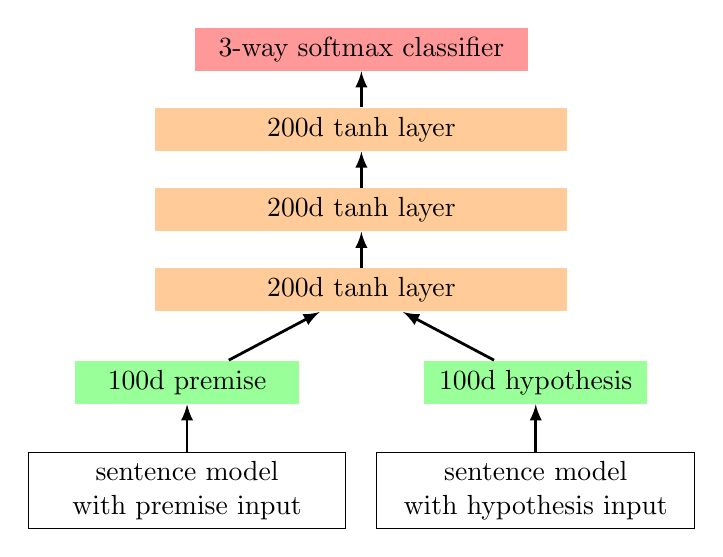
\begin{tikzpicture}
    \def\dx{21pt}
    \def\dy{29pt}

    \tikzstyle{label}=[text width=40mm,align=center]    
    \tikzstyle{softmax}=[fill=red!40,text width=40mm,align=center]
    \tikzstyle{preclass}=[fill=orange!40,text width=50mm,align=center]
    \tikzstyle{e}=[fill=green!40,text width=26mm,align=center]
    \tikzstyle{m}=[draw=black,text width=38mm,align=center]    
    
    \node[softmax]  (softmax) at (0*\dx,6*\dy) {3-way softmax classifier};
    \node[preclass]  (pc3) at (0*\dx,5*\dy) {200d $\tanh$ layer};
    \node[preclass]  (pc2) at (0*\dx,4*\dy) {200d $\tanh$ layer};
    \node[preclass]  (pc1) at (0*\dx,3*\dy) {200d $\tanh$ layer};
    \node[e]  (pe) at (-3*\dx,1.85*\dy) {100d premise};
    \node[e]  (he) at (3*\dx,1.85*\dy) {100d hypothesis};
    \node[m]  (pem) at (-3*\dx,0.5*\dy) {sentence model\\ with premise input};
    \node[m]  (hem) at (3*\dx,0.5*\dy) {sentence model\\ with hypothesis input};    
    
    \pgfsetarrowsend{latex}
    \tikzstyle{fwd} = [draw=black, line width=1pt]

          \draw [fwd] (pc3) -- (softmax);
          \draw [fwd] (pc2) -- (pc3);
          \draw [fwd] (pc1) -- (pc2);
          \draw [fwd] (pe) -- (pc1);
          \draw [fwd] (he) -- (pc1);
          \draw [fwd] (hem) -- (he);
          \draw [fwd] (pem) -- (pe);

  \end{tikzpicture}}
	
        \caption{The neural network classification architecture: for each sentence embedding model evaluated in \reftabs{tab:nnresults}{tab:transferresults}, two identical copies of the model are run with the two sentences as input, and their outputs are used as the two 100d inputs shown here.}
  \label{modelstructure}
\end{figure}

Our neural network classifier, depicted in \reffig{modelstructure} (and based on a one-layer model in \citealt{Bowman:Potts:Manning:2014}), is simply a stack of three 200d $\tanh$ layers, with the bottom layer taking the concatenated sentence representations as input and the top layer feeding a softmax classifier, all trained jointly with the sentence embedding model itself.

We test three sentence embedding models, each set to use 100d phrase and sentence embeddings. Our baseline sentence embedding model simply sums the embeddings of the words in each sentence. In addition, we experiment with two simple sequence embedding models: a plain RNN and an LSTM RNN \cite{hochreiter1997long}.

The word embeddings for all of the models are initialized with the 300d reference GloVe vectors (840B token version, \citealt{pennington2014glove}) and fine-tuned as part of training. In addition, all of the models use an additional $\tanh$ neural network layer to map these 300d embeddings into the lower-dimensional phrase and sentence embedding space. All of the models are randomly initialized using standard techniques and trained using AdaDelta \cite{zeiler2012adadelta} minibatch SGD until performance on the development set stops improving. We applied L2 regularization to all models, manually tuning the strength coefficient $\lambda$ for each, and additionally applied dropout \cite{srivastava2014dropout} to the inputs and outputs of the sentence embedding models (though not to its internal connections) with a fixed dropout rate. All models were implemented in a common framework for this paper, and the implementations will be made available at publication time.

\begin{table}
\begin{center}
\begin{tabular}{l@{\hskip \colspaceL}@{\hskip \colspaceL}c@{\hskip \colspaceL}c}
\toprule
\textbf{Sentence model} & \b{Train}  & \b{Test}\\
\midrule
\t{100d Sum of words}            & \t{79.3} & \t{75.3} \\
% scr/snlirc3d-snlirc3-only-l0.0001-dim100-ed300-td3-pen200-do0.9-0.9-co3-comp-1-dp1-gc5-lstminit5/stat_log
% 290500, dev 76.4, converged

\t{100d RNN}            & \t{73.1} & \t{72.2} \\	
% scr/snlirc3d-snlirc3-only-l0.0001-dim100-ed300-td3-pen200-do0.9-0.9-co3-comp3-dp1-gc5-lstminit5/stat_log
% 338500, dev 72.5, mostly converged

\t{100d LSTM RNN}            & \t{84.8} & \b{77.6} \\
% scr/snlirc3d-snlirc3-only-l3e-05-dim100-ed300-td3-pen200-do0.95-0.95-co3-comp2-dp1-gc5-lstminit5/stat_log
% 372000, dev 79.11, mostly converged

% \t{100d TreeRNN}            & \t{69?} & \t{69?} \\
% \t{50d TreeRNTN}            & \t{61?} & \t{60?} \\
% \t{100d LSTM TreeRNN}            & \t{72?} & \t{73?} \\
\bottomrule
\end{tabular}
\end{center}
% The caption
\caption{
\label{tab:nnresults}
Accuracy in 3-class classification on our training and test sets for each model.
}
\end{table}

The results are shown in \reftab{tab:nnresults}. The sum of words model performed slightly worse than the fundamentally similar lexicalized classifier---while the sum of words model can use pretrained word embeddings to better handle rare words, it lacks even the rudimentary sensitivity to word order that the lexicalized model's bigram features provide. Of the two RNN models, the LSTM's more robust ability to learn long-term dependencies serves it well, giving it a substantial advantage over the plain RNN, and  resulting in performance that is essentially equivalent to the lexicalized classifier on the test set (LSTM performance near the stopping iteration varies by up to 0.5\% between evaluation steps). While the lexicalized model fits the training set almost perfectly, the gap between train and test set accuracy is relatively small for all three neural network models, suggesting that research into significantly higher capacity versions of these models would be productive.

\subsection{Analysis and discussion}

\Reffig{fig:bowlearncurve} shows a learning curve for the LSTM and the lexicalized and unlexicalized feature-based models. It shows that the large size of the corpus is crucial to both the LSTM and the lexicalized model, and suggests that additional data would yield still better performance for both. In addition, though the LSTM and the lexicalized model show similar performance when trained on the current full corpus, the somewhat steeper slope for the LSTM hints that its ability to learn arbitrarily structured representations of sentence meaning may give it an advantage over the more constrained lexicalized model on still larger datasets.

% useful resource in the development of more sophisticated SE models

\Fig{new_lcc.pdf}{0.83}{bowlearncurve}{
A learning curve showing how the baseline classifiers and the LSTM perform when trained to convergence on varied amounts of training data. The y-axis starts near a random-chance accuracy of 33\%. The minibatch size of 64 that we used to tune the LSTM sets a lower bound on data for that model.}

% Insights 2: the learning curve for the unlexicalized classifier is sad
We were struck by the speed with which the lexicalized classifier outperforms its unlexicalized counterpart.
With only 100 training examples, the cross-bigram classifier is already performing better.
Empirically, we find that the top weighted features for the classifier
  trained on 100 examples tend to be high precision entailments;
  e.g.,
  \textit{playing} $\rightarrow$ \textit{outside}
  (most scenes are outdoors), \textit{a banana} $\rightarrow$
  \textit{person eating}.
If relatively few spurious entailments get high weight---as it appears
is the case---then it makes sense that, when these do fire, they
boost accuracy in identifying entailments.
  
There are revealing patterns in the errors common to all the models
considered here. Despite the large size of the training corpus and the
distributional information captured by GloVe initialization, many
lexical relationships are still misanalyzed, leading to incorrect
predictions of \ii{independent}, even for pairs that are common in the
training corpus like \word{beach}/\word{surf} and
\word{sprinter}/\word{runner}. Semantic mistakes at the phrasal level
(e.g., predicting contradiction for \word{A male is placing an order in a 
deli}/\word{A man buying a sandwich at a deli}) indicate
that additional attention to compositional semantics would pay off.
%
% Others that could replace the above:
% \word{Two teen girls relax on a black futon}/\word{Two young girls are sitting inside}
% \word{A male is placing an order in a deli}/\word{A man buying a sandwich at a deli}
% \word{A shopper buys cat food at a Walmart}/\word{A person shops for their pet at a store}
However, many of the persistent problems run deeper, to inferences
that depend on world knowledge and context-specific inferences, as in
the entailment pair \word{A race car driver leaps from a burning
  car}/\word{A race car driver escaping danger}, for which both
the lexicalized classifier and the LSTM predict \ii{neutral}. 
In other cases, the models' attempts to shortcut this kind of inference 
through lexical cues can lead them astray. 
Some of these examples have qualities
reminiscent of Winograd schemas \cite{Winograd:1972,Levesque:2013}. For
example, all the models wrongly predict
entailment for \word{A young girl throws sand toward the
  ocean}/\word{A girl can't stand the ocean}, presumably because of
distributional associations between \word{throws} and \word{can't
  stand}.

Analysis of the models' predictions also yields insights into the
extent to which they grapple with event and entity coreference. For
the most part, the original image prompts contained a focal element
that the caption writer identified with a syntactic subject, following
information structuring conventions associating subjects and topics in
English \cite{Ward04}. Our annotators generally followed suit, writing
sentences that, while structurally diverse, share topic/focus (theme/rheme)
structure with their premises.
This promotes a coherent, situation-specific construal of each sentence
pair. This is information that our models can easily take advantage
of, but it can lead them astray. For instance, all of them stumble
with the amusingly simple case \emph{A woman prepares ingredients for
  a bowl of soup}/\emph{A soup bowl prepares a woman}, in which prior
expectations about parallelism are not met. Another headline example
of this type is \emph{A man wearing padded arm protection is being
  bitten by a German shepherd dog}/\emph{A man bit a dog}, which all
the models wrongly diagnose as \ii{entailment}, though the sentences
report two very different stories. A model with access
to explicit information about syntactic or semantic structure should perform
better on cases like these.
% CP is a fan of ``headline'' -- newspaper theme -- so didn't delete.

\section{Transfer learning with SICK}

To the extent that successfully training a neural network model like our LSTM on SNLI forces that model to encode broadly accurate representations of English scene descriptions and to build an entailment classifier over those relations, we should expect it to be readily possible to adapt the trained model for use on other NLI tasks. In this section, we evaluate on the SICK entailment task using a simple transfer learning method \cite{pratt1991direct} and achieve competitive results.

\begin{table}
\begin{center}
\begin{tabular}{l@{\hskip \colspaceL}@{\hskip \colspaceL}r@{\hskip \colspaceL}r}
\toprule
\textbf{Training sets} & \b{Train}  & \b{Test}\\
\midrule
\t{Our data only}            & \t{42.0} & \t{46.7} \\
% scr/transfer5-sick-only-transfer-l0.0001-dim100-ed300-td3-pen200-do0.95-0.95-ws3-adi1-comp2-cdim1/stat_log
% Step 0, no learning intended after transfer
\t{SICK only}            & \t{100.0} & \t{71.3} \\
% From: ~/quant/transfer-sick-only-l0.0001-dim50-ed200-td3-pen100-do0.9-0.9-ws1-par0-comp2-cdim1/
\t{Our data and SICK (transfer)}            & \t{99.9} & \b{80.8} \\
% From: ~/quant/transfer5-sick-only-transfer-l0.0001-dim100-ed300-td3-pen200-do0.95-0.95-ws3-adi0-comp2-cdim1/stat_log
\bottomrule
\end{tabular}
\end{center}

\caption{\label{tab:transferresults}
LSTM 3-class accuracy on the SICK train and test sets under three training regimes.} 
% TODO (Gabor): Report training accuracy for the model trained on SICK.
\end{table}


To perform transfer, we take the parameters of the LSTM RNN model trained on SNLI and use them to initialize a new model, which is trained from that point only on the training portion of SICK. The only newly initialized parameters are softmax layer parameters and the embeddings for words that appear in SICK, but not in SNLI (which are populated with GloVe embeddings as above). We use the same model hyperparameters that were used to train the original model, with the exception of the L2 regularization strength, which is re-tuned. We additionally transfer the accumulators that are used by AdaDelta to set the learning rates. This lowers the starting learning rates, and is intended to ensure that the model does not learn too quickly in its first few epochs after transfer and destroy the knowledge accumulated in the pre-transfer phase of training.

The results are shown in \reftab{tab:transferresults}. Training on SICK alone yields poor performance, and the model trained on SNLI fails when tested on SICK data, labeling more \ii{neutral} examples as \ii{contradiction}s than correctly, possibly as a result of subtle differences in how the labeling task was presented. In contrast, transferring SNLI representations to SICK yields the best performance yet reported for an unaugmented neural network model, surpasses the available EOP models, and approaches both the overall state of the art at 84.6\% \cite{lai2014illinois} and the 84\% level of interannotator agreement, which likely represents an approximate performance ceiling. This suggests that the introduction of a large high-quality corpus makes it  possible to train representation-learning models for sentence meaning that are competitive with the best hand-engineered models on inference tasks.

We attempted to apply this same transfer evaluation technique to the RTE-3 challenge, but found that the small training set (800 examples) did not allow the model to adapt to the unfamiliar genre of text used in that corpus, such that no training configuration yielded competitive performance.
Further research on effective transfer learning on small data sets with neural models might facilitate improvements here.


% A woman prepares ingredients for a bowl of soup.	A soup bowl prepares a woman.


% \section{NLI data and transfer learning}\label{sec:transfer}

We argue that for a sentence representation to provide the information necessary to reliably perform NLI classification, it must contain a faithful and thorough description of the sentence's meaning. This claim has a readily testable consequence: the knowledge that a representation learning system learns when it is trained on SNLI should transfer well to any other task that involves understanding sentence meaning, at least to the extent that the style of language used in that task is broadly similar to the style of SNLI. To test this, we perform transfer learning \cite{pratt1991direct} experiments on four other tasks, in which models are initialized using the parameters of an LSTM RNN-based model trained on SNLI (as in \S\ref{sentence-embedding}) and then trained to convergence on the target tasks. 

We first evaluate on SICK (\citealt{marelli2014sick}), the smaller entailment corpus ours was modeled on, training on the standard 4.5k training sentence pairs. We then evaluate on SUBJ (\citealt{pang2004sentimental}), a two-way sentence classification task, using 5-fold cross-validation over the 10k sentences. We next evaluate on the Stanford Sentiment Treebank (SST; \citealt{socher2013acl1}), a five-way sentiment classification task with labels for both phrases and sentences. We train on both types of label within the 8.5k sentence training set and test on only the sentence-level labels in the test set. We finally evaluate on PragBank, an 800 example 6-way sentence classification task focused on veridicality. \todo{Cite} ....
\noindent\todo{Pick best 2-3 tasks.}

We use pretrained parameters for all of the LSTM parameters, pretrained parameters for the $\tanh$ layers in the classifier stack, and pretrained embeddings for all of the words that occurred in both corpora, randomly initializing only the softmax layer and the remaining word embeddings. In order to use this strategy in sentence classification tasks, we pass the classifier the embedding of the sentence to be classified in the hypothesis input position, as well as a zero vector in the premise input position. After transfer, we re-initialize the accumulators in AdaDelta to re-set the learning rates to high values. We additionally use L2 regularization with each task, separately tuning the regularization strength on the transfer model and the corresponding baseline model without transfer.

\noindent\todo{Do we still want to re-initialize LRs?}


\begin{table}
\begin{center}
\begin{tabular}{l@{\hskip \colspaceL}c@{\hskip \colspaceS}c@{\hskip \colspaceS}c@{\hskip \colspaceS}c@{\hskip \colspaceS}c}
\hline
\textbf{Corpus} & \multicolumn{2}{c}{\b{Train Acc.}} &\multicolumn{3}{c}{ \b{Test Acc.}} \\
 & \t{cold start} & \t{transfer} & \t{cold start} & \t{transfer} & \t{SotA} \\
\hline
\t{SICK}            & \t{100} & \t{99} & \t{71.3?} & \t{80.1?} & \t{84.5} \\
\t{SUBJ}          & \t{??.?} & \t{??.?} & \t{90?} & \t{91?}& \t{95.5} \\
\t{SST}          & \t{??.?} & \t{??.?} & \t{43?} & \t{42?} & \t{50.6}\\
\t{PragBank}          & \t{??.?} & \t{??.?} & \t{50} & \t{56}& \t{~75} \\
\hline
\end{tabular}
\end{center}

\caption{\label{tab:transferresults}
The performance of an LSTM RNN model on four tasks under both a random initialization and a transfer initialization copied from a model trained on SNLI. All figures are classification accuracy, except for PragBank, where report macroaveraged F1 to enable comparison with existing results on that task. \todo{Final numbers.}} 

\end{table}

The final column shows the state of the art results from \citealt{lai2014illinois}, \citealt{zhao2015self}, \citealt{tai2015improved}, and \todo{CITE}.

The results are shown in \tabref{tab:transferresults}. For each task, the transfer model is compared with a model that was initialized randomly as normal. Note that \todo{something interesting happens}. Within the domain of NLI, our transfer model shows the best number yet reported on SICK for a fully-learned model, and approaches the overall state of the art (and to the 84\% level of interannotator agreement, a likely performance ceiling), while the randomly initialized model performs poorly. This suggests that the introduction of a large high-quality corpus makes it newly possible to train representation learning models for sentence meaning of a level of quality that is competitive with the best hand-engineered models on semantically sophisticated tasks.

\noindent\todo{something about SotA on the other tasks.}

\label{sec:conclusion}
We introduce a novel neural network architecture, the Synchronized Spectral CNN (SyncSpecCNN), for semantic annotation on 3D shape graphs. To share coefficients and conduct multi-scale analysis in different parts of a single shape graph, we introduce a spectral parametrization of dilated convolutional kernels. To allow parameter sharing across related but different shapes that may be represented by very different graphs, we introduce a spectral transformer network to synchronize different spectral domains. The effectiveness of different components in our network is validated through extensive experiments. Jointly these contributions lead to state-of-the-art performance on various semantic annotation tasks including 3D shape part segmentation and 3D keypoint prediction.

\subsubsection*{Acknowledgments}

%
We gratefully acknowledge support from %
a Google Faculty Research Award, %
a gift from Bloomberg L.P., 
the Defense Advanced Research Projects Agency (DARPA) Deep Exploration and Filtering of Text (DEFT) Program under Air Force Research Laboratory (AFRL) contract no.~FA8750-13-2-0040,
the National Science Foundation under grant no.~IIS 1159679, and %
the Department of the Navy, Office of Naval Research, under grant no.~N00014-10-1-0109.
%
Any opinions, findings, and conclusions or recommendations expressed in this material are those of the authors and do not necessarily reflect the views of 
Google, 
Bloomberg L.P.,
DARPA,
AFRL
NSF, 
ONR, or 
the US government. We also thank our many excellent Mechanical Turk contributors.



% Do not number the acknowledgment section.

\bibliographystyle{acl}
% We get two pages for references, so I suggest leaving the page
% numbers in -- it's not worth the time to remove them, and they
% could be helpful to people!
%\noindent\todo{Omit page numbers for proceedings in bib?}
\bibliography{MLSemantics} 

\end{document}
